% Unofficial University of Cambridge Poster Template
% https://github.com/andiac/gemini-cam
% a fork of https://github.com/anishathalye/gemini
% also refer to https://github.com/k4rtik/uchicago-poster

\documentclass[final]{beamer}

% ====================
% Packages
% ====================

\usepackage[T1]{fontenc}
\usepackage{lmodern}
\usepackage[orientation=portrait,size=a1]{beamerposter}
\usetheme{gemini}
\usecolortheme{nott}
\usepackage{graphicx}
\usepackage{booktabs}
\usepackage{tikz}
\usepackage{pgfplots}
\pgfplotsset{compat=1.14}
\usepackage{anyfontsize}
\usepackage{kotex}
\usepackage{amsmath}
\usepackage{mathtools}
\usepackage{amssymb}
\usepackage[labelformat=empty]{caption}
\usepackage{subcaption}

\captionsetup[subfigure]{labelformat=empty}

% ====================
% Lengths
% ====================

% If you have N columns, choose \sepwidth and \colwidth such that
% (N+1)*\sepwidth + N*\colwidth = \paperwidth
\newlength{\sepwidth}
\newlength{\colwidth}
% \setlength{\sepwidth}{0.025\paperwidth}
% \setlength{\colwidth}{0.45\paperwidth}

% \newcommand{\separatorcolumn}{\begin{column}{\sepwidth}\end{column}}


% ====================
% Title
% ====================

\title{Classifying Theta-Curves and Handcuff Graphs up to 7 Crossing by Arc Index(가제)}

\author{Cho Eunchan \inst{1} \and Jeongwon Shin \inst{1} \and Boyeon Seo \inst{1} \and Minho Choi \inst{1} \and Kim Hun \inst{2} \and 진교택 \inst{3} \and 이재원 \inst{4}}

\institute[shortinst]{\inst{1} Researcher, Korea Science Academy of KAIST \samelineand \inst{2} Supervisor, Another Institute \samelineand \inst{3} Co-Supervisor, asdf \samelineand \inst{4} Assistant, asdf \samelineand}

% ====================
% Footer (optional)
% ====================

\footercontent{
  \href{https://utfpr.edu.br/ct/ppgca}{utfpr.edu.br/ct/ppgca} \hfill
  Mostra de Trabalhos do PPGCA --- TechTalks 2024 \hfill
  \href{mailto:ppgca-ct@utfpr.edu.br}{ppgca-ct@utfpr.edu.br}}
% (can be left out to remove footer)


% ====================
% Logo (optional)
% ====================

% use this to include logos on the left and/or right side of the header:
% \logoright{
\includegraphics[height=2.5cm]{logos/utfpr-logo.png}}
% \logoleft{\hspace{20ex}
\includegraphics[height=3.5cm]{logos/ppgca-logo.png}}

% ====================
% Body
% ====================



\begin{document}

% Refer to https://github.com/k4rtik/uchicago-poster
% logo: https://www.cam.ac.uk/brand-resources/about-the-logo/logo-downloads
% \addtobeamertemplate{headline}{}
% {
%     \begin{tikzpicture}[remember picture,overlay]
%       \node [anchor=north west, inner sep=3cm] at ([xshift=-2.5cm,yshift=1.75cm]current page.north west)
%       {\includegraphics[height=7cm]{logos/unott-logo.eps}}; 
%     \end{tikzpicture}
% }

\begin{frame}[t]
% \begin{columns}[t]
% \separatorcolumn

% \begin{column}{\colwidth}
\begin{columns}[t]
  \column{0.33\textwidth}
  \begin{block}{Definitions}
    \begin{itemize}
      \item \textbf{Theta-curve} is a spatial knot on 3-sphere which has 2 vertices and 3 edges.
      In the projection of the theta-curve, the section where theta-curve meets itself is named \textbf{crossing}.
      If the one theta-curve and other theta-curve's continuous transform of the graph is same, these curves are \textbf{equivalent}.
      To transform a projection of theta-curve, the \textbf{generalized Reidemeister move} is used.
      \item \textbf{Handcuff graph} consists of two loops and an edge joining the loops.
      \item The \textbf{grid diagram} is made of horizontal lines and vertical lines, and vertical lines are always on top of horizontal lines.
      Except the vertices, two points that are bent vertically should be on each horizontal and vertical lines.
      The \textbf{Cromwell matrix} of theta-curve and handcuff graphs is the matrix made of 0 and 1.
      Except 2 rows, each row and columns has exactly two 1s, and for 2 rows, there are exactly three 1s.
      If the 1s are connected by horizontal and vertical lines, it leads to the grid diagram.
      The arc presentation can be expressed by grid diagram and vice versa.
      They are in one-to-one correspondence.
      Also, if the number of half planes are $\alpha$ on minimal arc presentation, the size of corresponding grid diagram is $(\alpha - 1) \times \alpha$.\\

    \end{itemize}
  \end{block}
  \column{0.33\textwidth}
  \begin{block}{Classifying Theta-Curves and Handcuff Graphs by Determinant}
      $\mathbf{Theorem.}$ The given THC-Cromwell matrix is theta-curve if and only if determinant of the H-deletion matrix is $\pm 1$.
      The given THC-Cromwell matrix is handcuff graph if and only if determinant of the H-deletion matrix is 0 or $\pm 2$.
  \end{block}
  \column{0.33\textwidth}
  \begin{block}{새로운 거}

    This block catches your eye, so \textbf{important stuff} should probably go
    here.

    Curabitur eu libero vehicula, cursus est fringilla, luctus est. Morbi
    consectetur mauris quam, at finibus elit auctor ac. Aliquam erat volutpat.
    Aenean at nisl ut ex ullamcorper eleifend et eu augue. Aenean quis velit
    tristique odio convallis ultrices a ac odio.

    \begin{itemize}
      \item \textbf{Fusce dapibus tellus} vel tellus semper finibus. In
        consequat, nibh sed mattis luctus, augue diam fermentum lectus.
      \item \textbf{In euismod erat metus} non ex. Vestibulum luctus augue in
        mi condimentum, at sollicitudin lorem viverra.
      \item \textbf{Suspendisse vulputate} mauris vel placerat consectetur.
        Mauris semper, purus ac hendrerit molestie, elit mi dignissim odio, in
        suscipit felis sapien vel ex.
    \end{itemize}

    Aenean tincidunt risus eros, at gravida lorem sagittis vel. Vestibulum ante
    ipsum primis in faucibus orci luctus et ultrices posuere cubilia Curae.

  \end{block}
\end{columns}

 \begin{alertblock}{Grid Diagram of the Theta-Curves and Handcuff Graphs Up to 7 Crossings}
  \hspace{1cm}
  \begin{columns}[t]
  \begin{column}{0.5\textwidth}
  \begin{alertblock}{Theta-Curves}
  \hspace{1cm}
  \begin{figure}
    \begin{subfigure}{0.075\textwidth}
    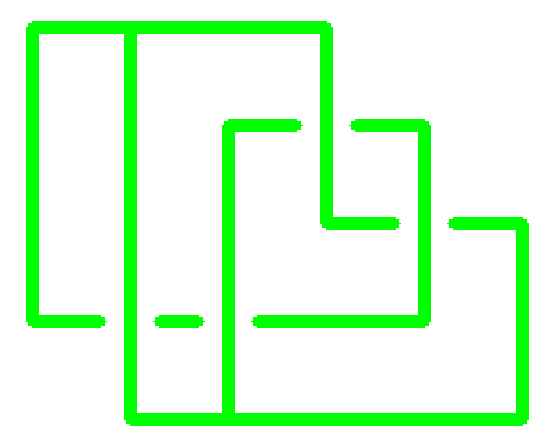
\includegraphics[width=\columnwidth]{C:/Users/io25j/Pictures/backup/documents/GitHub/R-E/Midterm_Poster/grid_diagram/theta_3_1.png}
    \caption{$3_1$} 
    \end{subfigure}
    \begin{subfigure}{0.075\textwidth}
    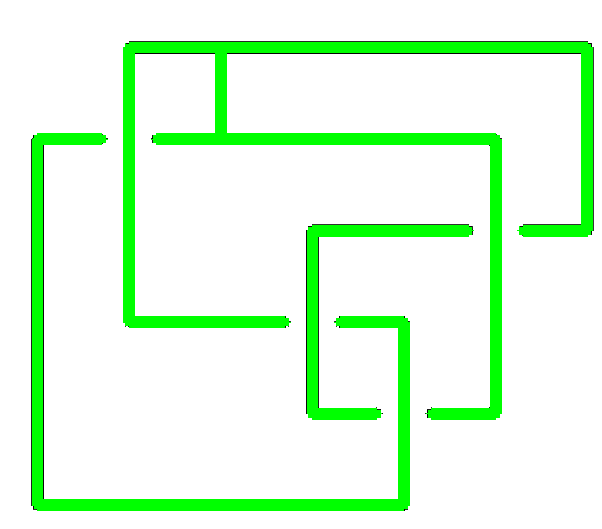
\includegraphics[width=\columnwidth]{C:/Users/io25j/Pictures/backup/documents/GitHub/R-E/Midterm_Poster/grid_diagram/theta_4_1.png}
    \caption{$4_1$} 
    \end{subfigure}
    \begin{subfigure}{0.075\textwidth}
    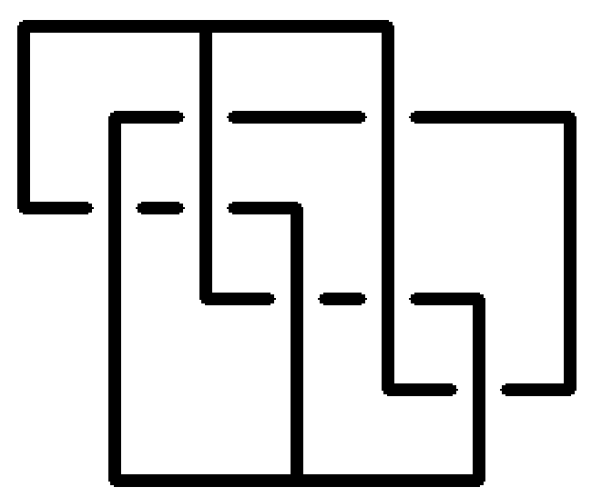
\includegraphics[width=\columnwidth]{C:/Users/io25j/Pictures/backup/documents/GitHub/R-E/Midterm_Poster/grid_diagram/theta_5_1.png}
    \caption{$5_1$}
    \end{subfigure}
    \begin{subfigure}{0.075\textwidth}
    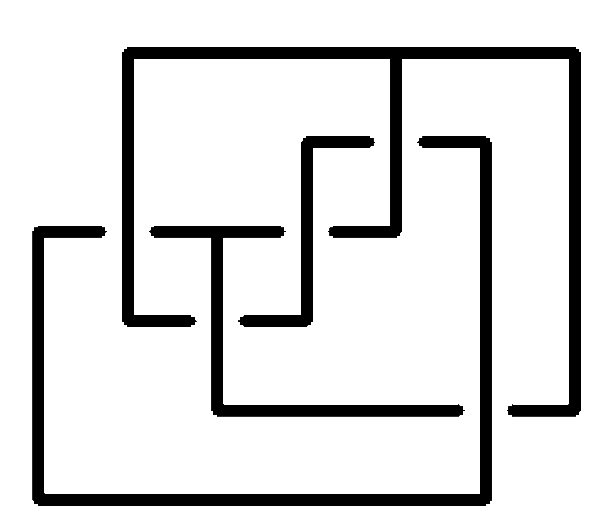
\includegraphics[width=\columnwidth]{C:/Users/io25j/Pictures/backup/documents/GitHub/R-E/Midterm_Poster/grid_diagram/theta_5_2.png}
    \caption{$5_2$} 
    \end{subfigure}
    \begin{subfigure}{0.075\textwidth}
    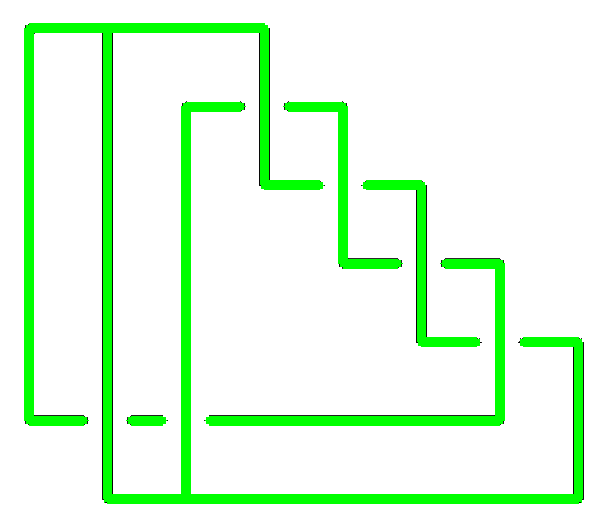
\includegraphics[width=\columnwidth]{C:/Users/io25j/Pictures/backup/documents/GitHub/R-E/Midterm_Poster/grid_diagram/theta_5_3.png}
    \caption{$5_3$}
    \end{subfigure}
    \begin{subfigure}{0.075\textwidth}
    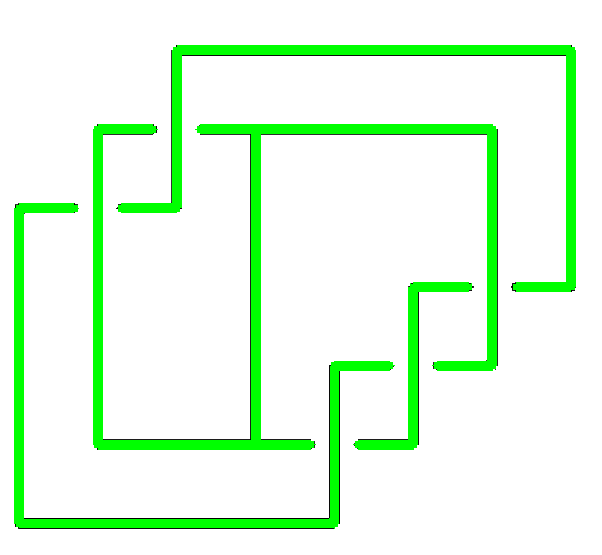
\includegraphics[width=\columnwidth]{C:/Users/io25j/Pictures/backup/documents/GitHub/R-E/Midterm_Poster/grid_diagram/theta_5_4.png}
    \caption{$5_4$} 
    \end{subfigure}
    \begin{subfigure}{0.075\textwidth}
    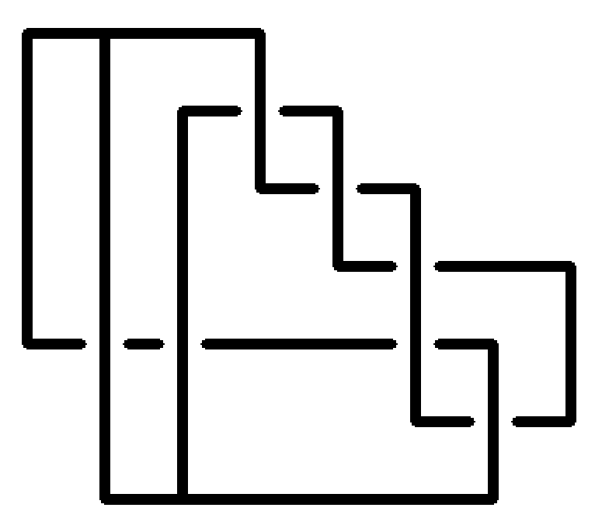
\includegraphics[width=\columnwidth]{C:/Users/io25j/Pictures/backup/documents/GitHub/R-E/Midterm_Poster/grid_diagram/theta_5_5.png}
    \caption{$5_5$} 
    \end{subfigure}
    \begin{subfigure}{0.075\textwidth}
    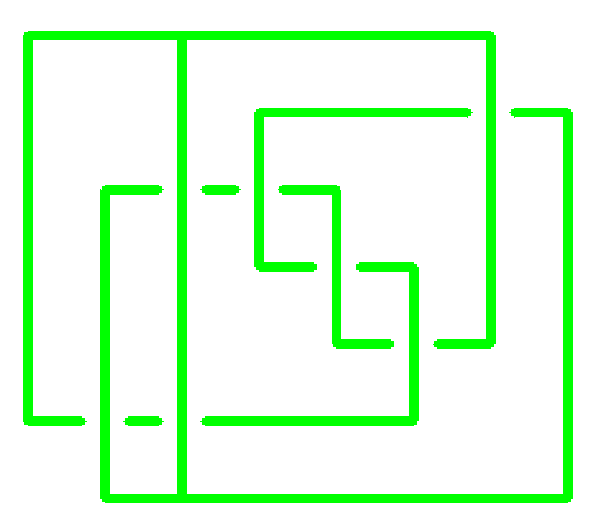
\includegraphics[width=\columnwidth]{C:/Users/io25j/Pictures/backup/documents/GitHub/R-E/Midterm_Poster/grid_diagram/theta_5_6.png}
    \caption{$5_6$} 
    \end{subfigure}
    \begin{subfigure}{0.075\textwidth}
    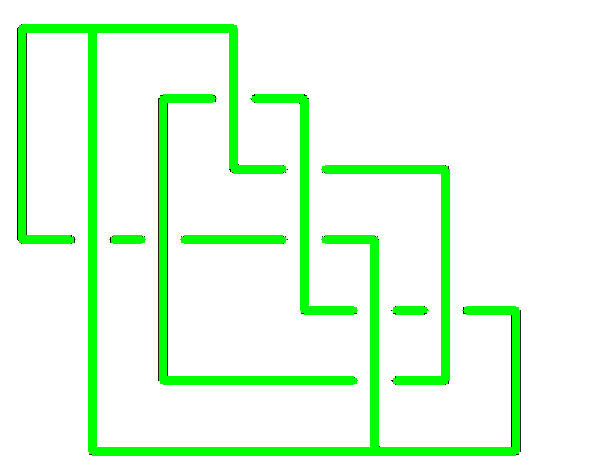
\includegraphics[width=\columnwidth]{C:/Users/io25j/Pictures/backup/documents/GitHub/R-E/Midterm_Poster/grid_diagram/theta_5_7.png}
    \caption{$5_7$} 
    \end{subfigure}
    \begin{subfigure}{0.075\textwidth}
    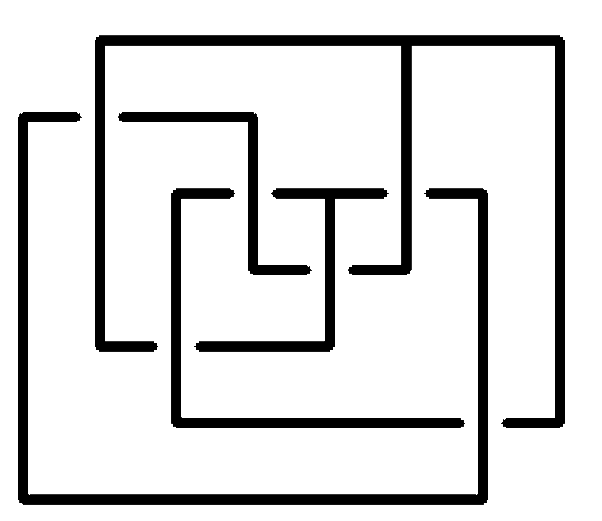
\includegraphics[width=\columnwidth]{C:/Users/io25j/Pictures/backup/documents/GitHub/R-E/Midterm_Poster/grid_diagram/theta_6_1.png}
    \caption{$6_1$} 
    \end{subfigure}
    \begin{subfigure}{0.075\textwidth}
    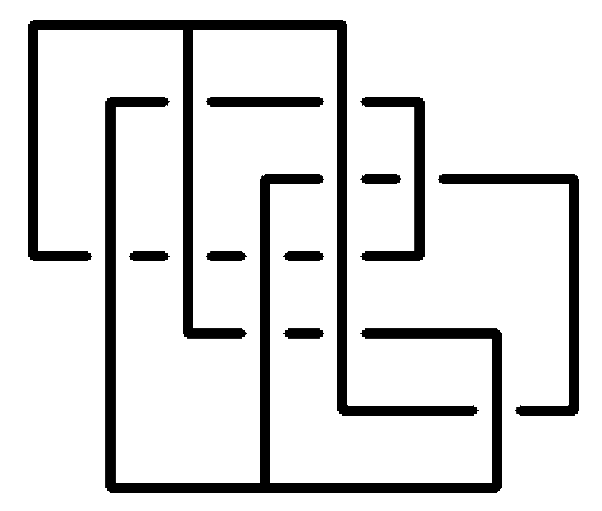
\includegraphics[width=\columnwidth]{C:/Users/io25j/Pictures/backup/documents/GitHub/R-E/Midterm_Poster/grid_diagram/theta_6_2.png}
    \caption{$6_2$} 
    \end{subfigure}
    \begin{subfigure}{0.075\textwidth}
    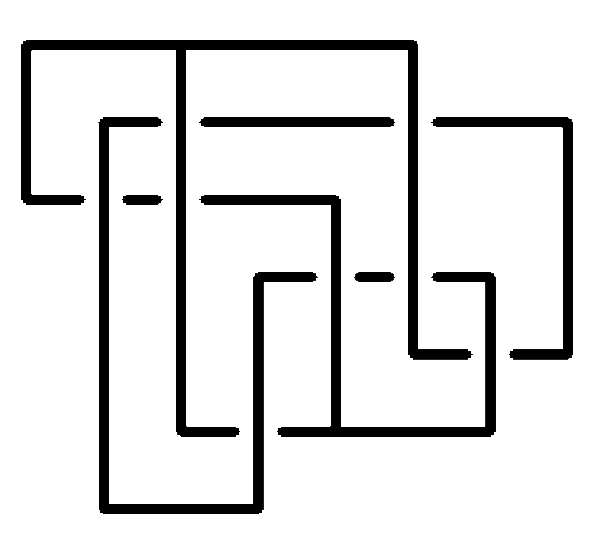
\includegraphics[width=\columnwidth]{C:/Users/io25j/Pictures/backup/documents/GitHub/R-E/Midterm_Poster/grid_diagram/theta_6_3.png}
    \caption{$6_3$} 
    \end{subfigure}
    \begin{subfigure}{0.075\textwidth}
    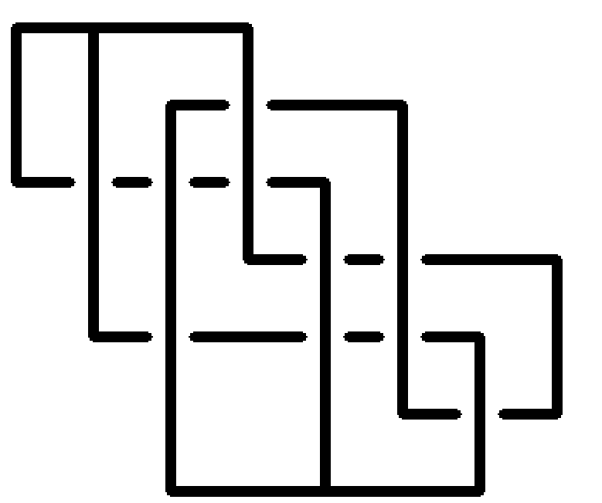
\includegraphics[width=\columnwidth]{C:/Users/io25j/Pictures/backup/documents/GitHub/R-E/Midterm_Poster/grid_diagram/theta_6_4.png}
    \caption{$6_4$} 
    \end{subfigure}
    \begin{subfigure}{0.075\textwidth}
    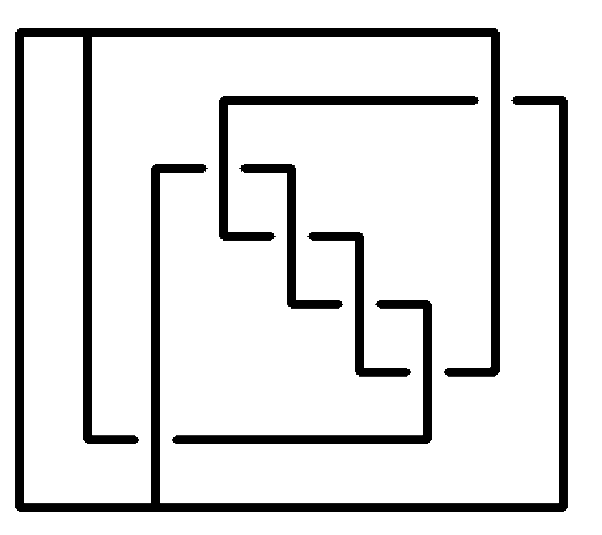
\includegraphics[width=\columnwidth]{C:/Users/io25j/Pictures/backup/documents/GitHub/R-E/Midterm_Poster/grid_diagram/theta_6_5.png}
    \caption{$6_5$} 
    \end{subfigure}
    \begin{subfigure}{0.075\textwidth}
    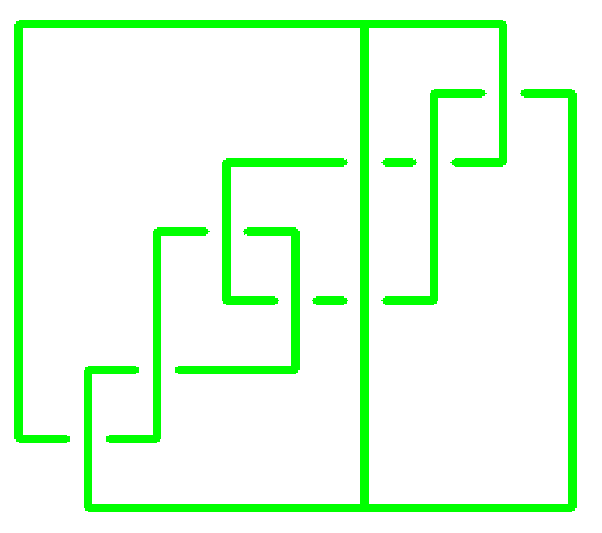
\includegraphics[width=\columnwidth]{C:/Users/io25j/Pictures/backup/documents/GitHub/R-E/Midterm_Poster/grid_diagram/theta_6_6.png}
    \caption{$6_6$} 
    \end{subfigure}
    \begin{subfigure}{0.075\textwidth}
    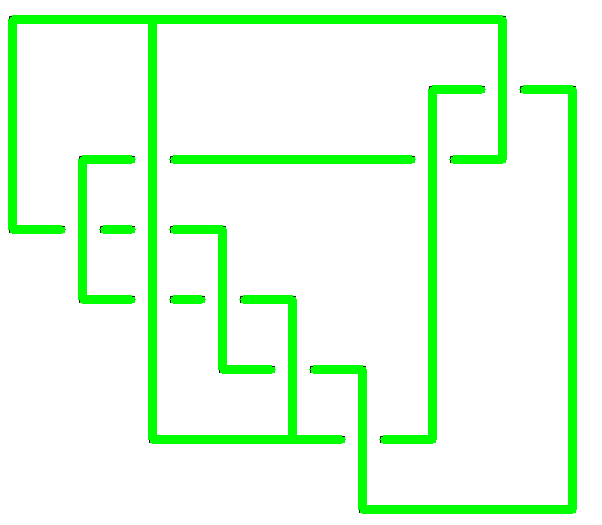
\includegraphics[width=\columnwidth]{C:/Users/io25j/Pictures/backup/documents/GitHub/R-E/Midterm_Poster/grid_diagram/theta_6_7.png}
    \caption{$6_7$} 
    \end{subfigure}
      \begin{subfigure}{0.075\textwidth}
    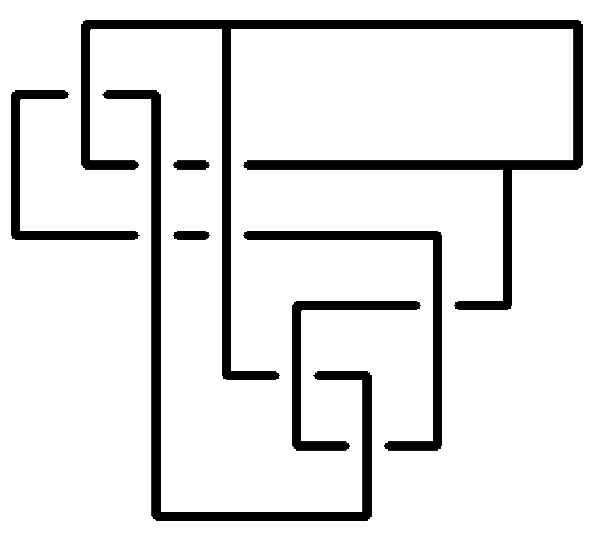
\includegraphics[width=\columnwidth]{C:/Users/io25j/Pictures/backup/documents/GitHub/R-E/Midterm_Poster/grid_diagram/theta_6_8.png}
    \caption{$6_8$} 
    \end{subfigure}
    \begin{subfigure}{0.075\textwidth}
    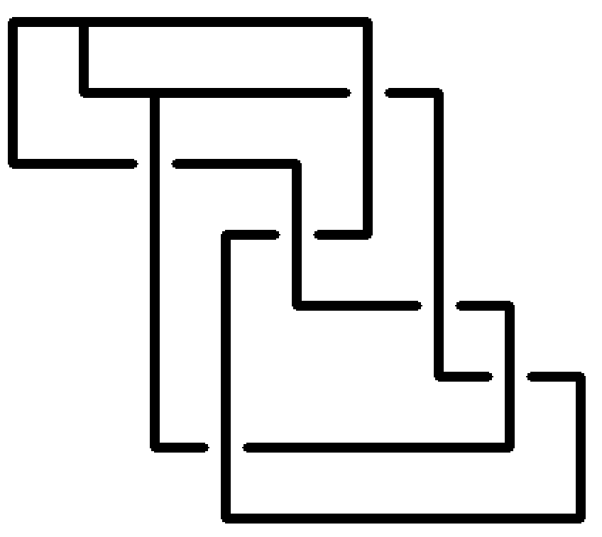
\includegraphics[width=\columnwidth]{C:/Users/io25j/Pictures/backup/documents/GitHub/R-E/Midterm_Poster/grid_diagram/theta_6_9.png}
    \caption{$6_9$} 
    \end{subfigure}
    \begin{subfigure}{0.075\textwidth}
    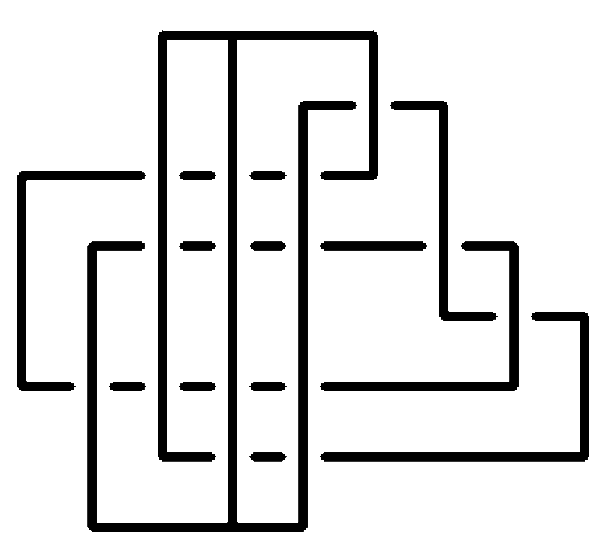
\includegraphics[width=\columnwidth]{C:/Users/io25j/Pictures/backup/documents/GitHub/R-E/Midterm_Poster/grid_diagram/theta_6_10.png}
    \caption{$6_{10}$} 
    \end{subfigure}
    \begin{subfigure}{0.075\textwidth}
    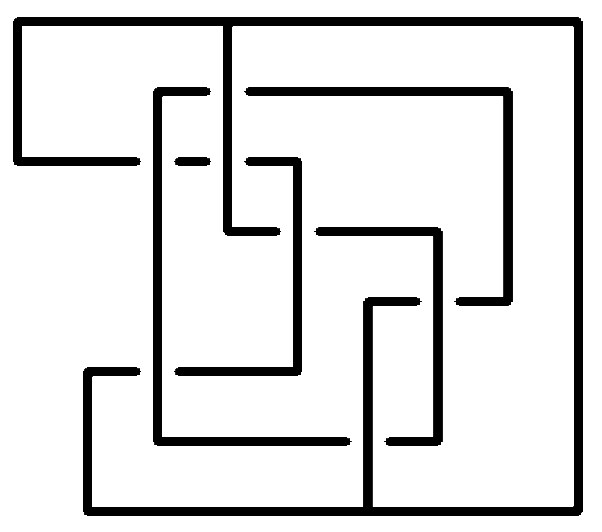
\includegraphics[width=\columnwidth]{C:/Users/io25j/Pictures/backup/documents/GitHub/R-E/Midterm_Poster/grid_diagram/theta_6_11.png}
    \caption{$6_{11}$} 
    \end{subfigure}
    \begin{subfigure}{0.075\textwidth}
    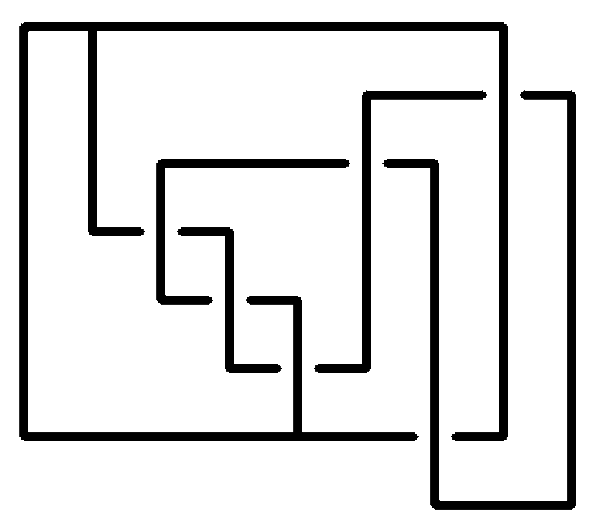
\includegraphics[width=\columnwidth]{C:/Users/io25j/Pictures/backup/documents/GitHub/R-E/Midterm_Poster/grid_diagram/theta_6_12.png}
    \caption{$6_{12}$} 
    \end{subfigure}
    \begin{subfigure}{0.075\textwidth}
    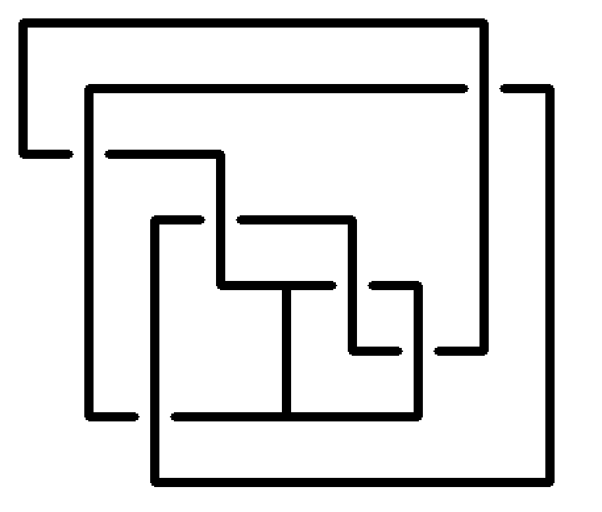
\includegraphics[width=\columnwidth]{C:/Users/io25j/Pictures/backup/documents/GitHub/R-E/Midterm_Poster/grid_diagram/theta_6_13.png}
    \caption{$6_{13}$} 
    \end{subfigure}
    \begin{subfigure}{0.075\textwidth}
    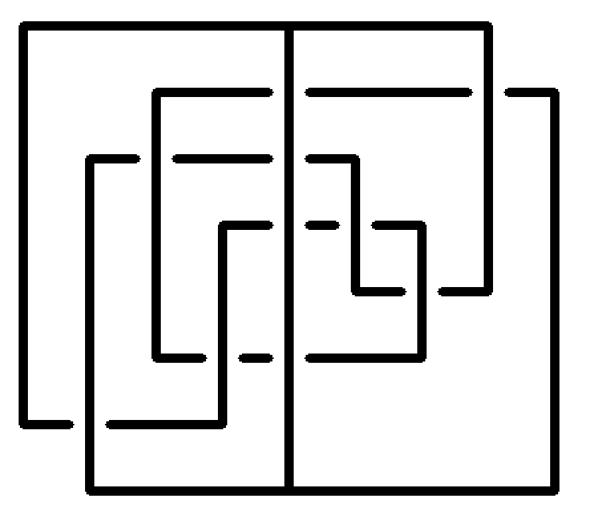
\includegraphics[width=\columnwidth]{C:/Users/io25j/Pictures/backup/documents/GitHub/R-E/Midterm_Poster/grid_diagram/theta_6_14.png}
    \caption{$6_{14}$} 
    \end{subfigure}
    \begin{subfigure}{0.075\textwidth}
    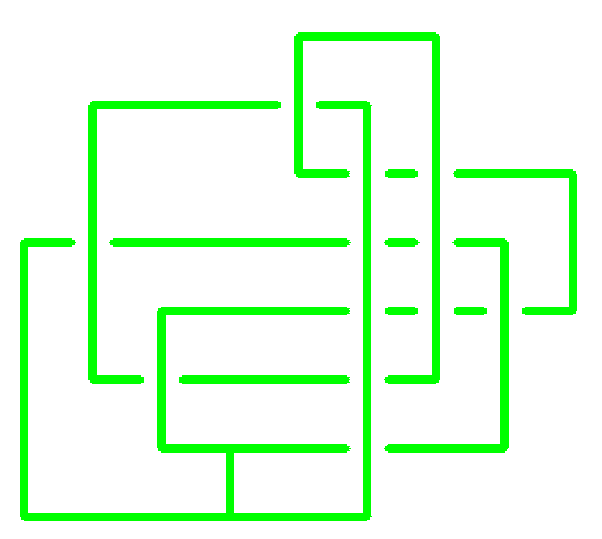
\includegraphics[width=\columnwidth]{C:/Users/io25j/Pictures/backup/documents/GitHub/R-E/Midterm_Poster/grid_diagram/theta_6_15.png}
    \caption{$6_{15}$} 
    \end{subfigure}
    \begin{subfigure}{0.075\textwidth}
    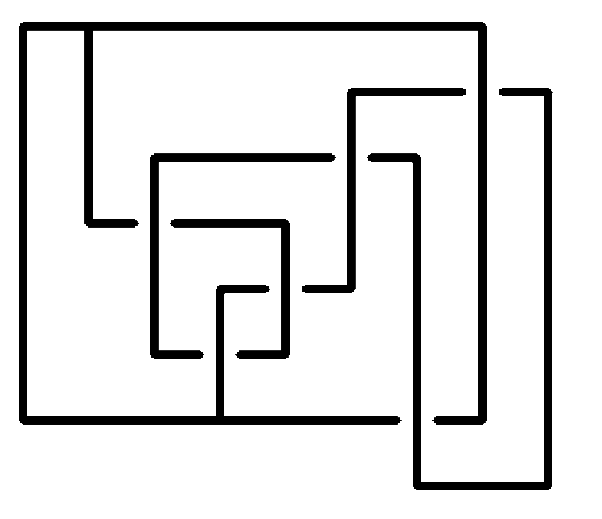
\includegraphics[width=\columnwidth]{C:/Users/io25j/Pictures/backup/documents/GitHub/R-E/Midterm_Poster/grid_diagram/theta_6_16.png}
    \caption{$6_{16}$} 
    \end{subfigure}
    \begin{subfigure}{0.075\textwidth}
    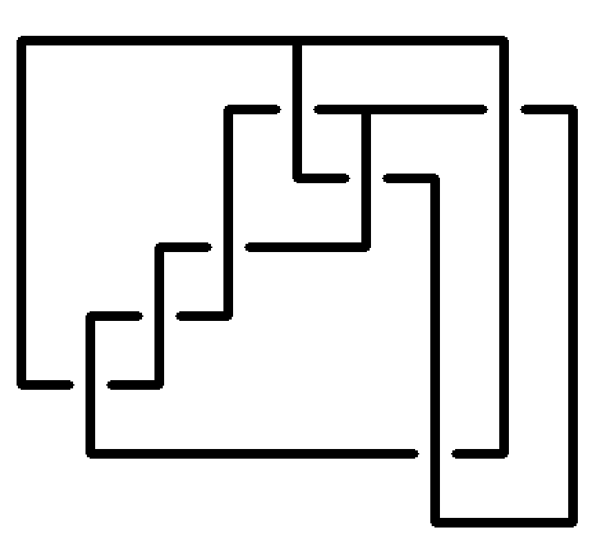
\includegraphics[width=\columnwidth]{C:/Users/io25j/Pictures/backup/documents/GitHub/R-E/Midterm_Poster/grid_diagram/theta_7_1.png}
    \caption{$7_{1}$} 
    \end{subfigure}
    \begin{subfigure}{0.075\textwidth}
    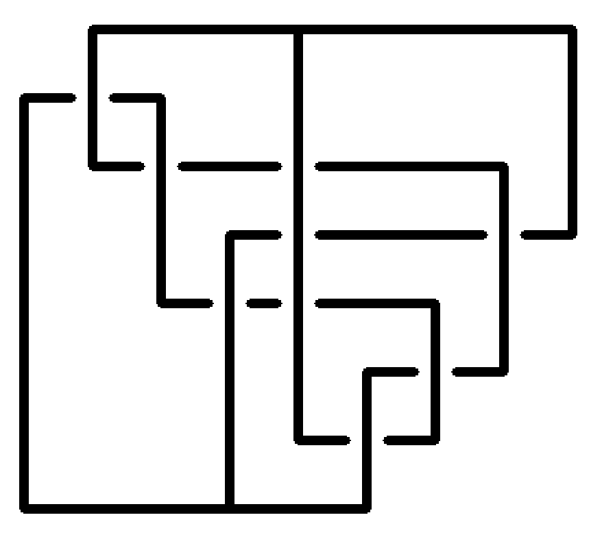
\includegraphics[width=\columnwidth]{C:/Users/io25j/Pictures/backup/documents/GitHub/R-E/Midterm_Poster/grid_diagram/theta_7_2.png}
    \caption{$7_{2}$} 
    \end{subfigure}
    \begin{subfigure}{0.075\textwidth}
    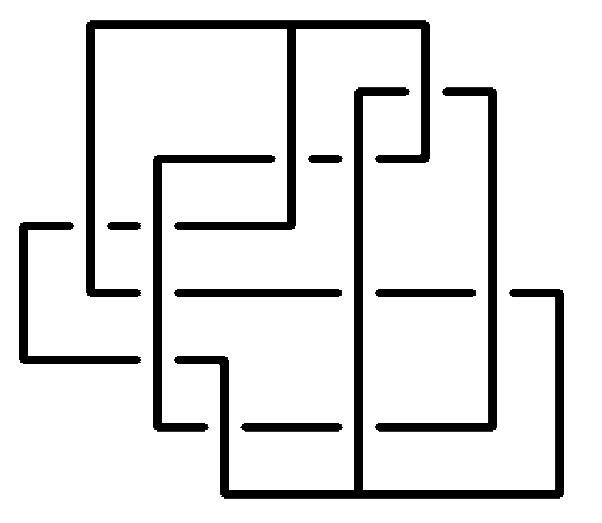
\includegraphics[width=\columnwidth]{C:/Users/io25j/Pictures/backup/documents/GitHub/R-E/Midterm_Poster/grid_diagram/theta_7_3.png}
    \caption{$7_{3}$} 
    \end{subfigure}
    \begin{subfigure}{0.075\textwidth}
    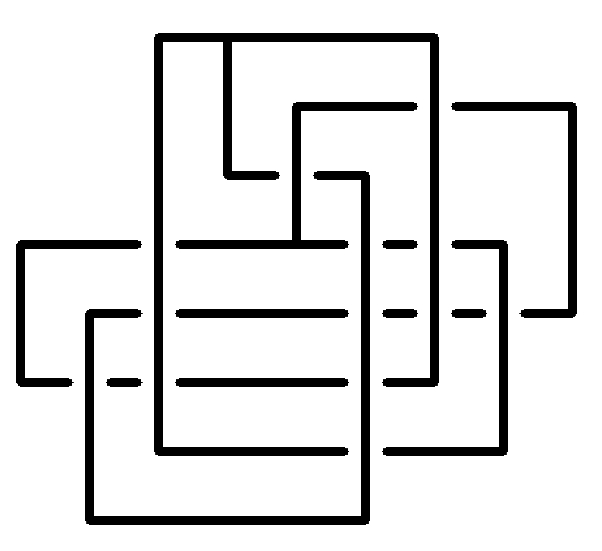
\includegraphics[width=\columnwidth]{C:/Users/io25j/Pictures/backup/documents/GitHub/R-E/Midterm_Poster/grid_diagram/theta_7_4.png}
    \caption{$7_{4}$} 
    \end{subfigure}
    \begin{subfigure}{0.075\textwidth}
    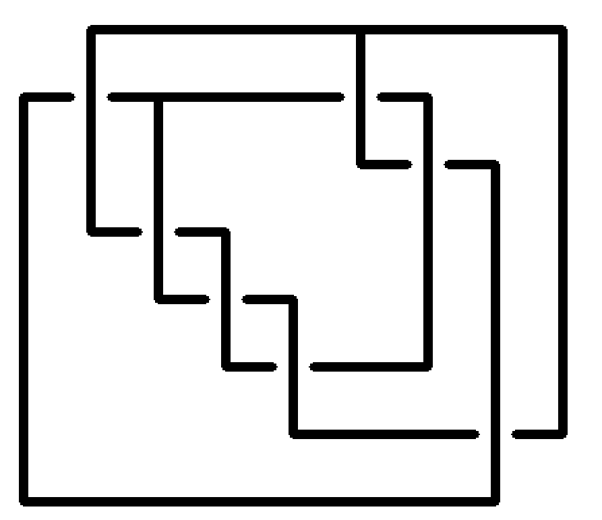
\includegraphics[width=\columnwidth]{C:/Users/io25j/Pictures/backup/documents/GitHub/R-E/Midterm_Poster/grid_diagram/theta_7_5.png}
    \caption{$7_{5}$} 
    \end{subfigure}
    \begin{subfigure}{0.075\textwidth}
    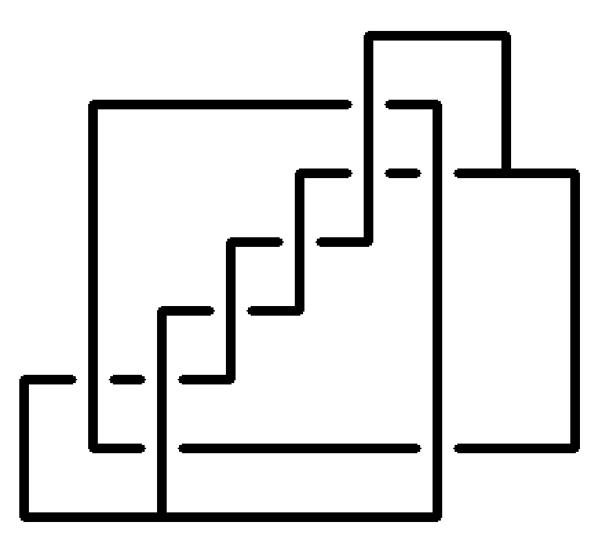
\includegraphics[width=\columnwidth]{C:/Users/io25j/Pictures/backup/documents/GitHub/R-E/Midterm_Poster/grid_diagram/theta_7_6.png}
    \caption{$7_{6}$} 
    \end{subfigure}
    \begin{subfigure}{0.075\textwidth}
    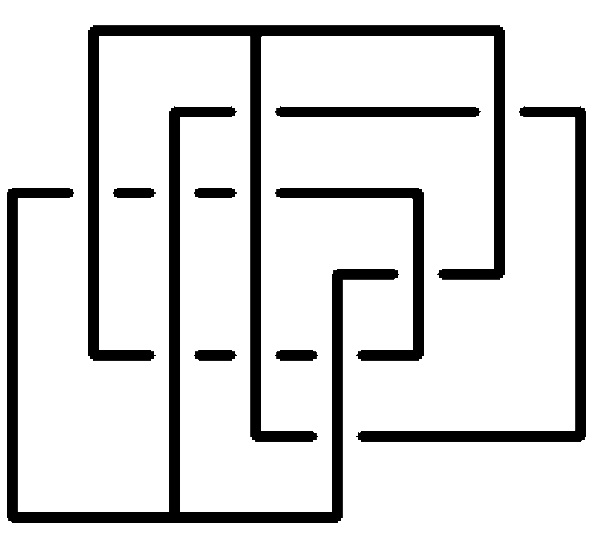
\includegraphics[width=\columnwidth]{C:/Users/io25j/Pictures/backup/documents/GitHub/R-E/Midterm_Poster/grid_diagram/theta_7_7.png}
    \caption{$7_{7}$} 
    \end{subfigure}
    \begin{subfigure}{0.075\textwidth}
    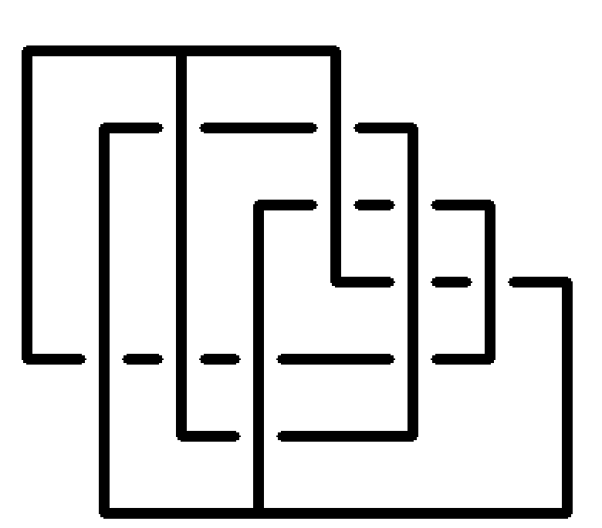
\includegraphics[width=\columnwidth]{C:/Users/io25j/Pictures/backup/documents/GitHub/R-E/Midterm_Poster/grid_diagram/theta_7_8.png}
    \caption{$7_{8}$} 
    \end{subfigure}
    \begin{subfigure}{0.075\textwidth}
    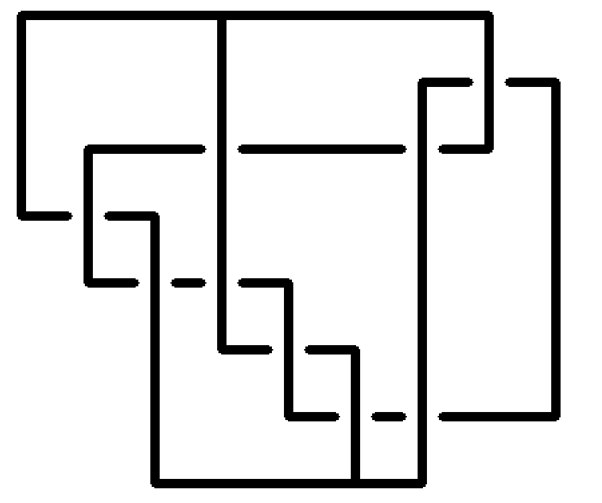
\includegraphics[width=\columnwidth]{C:/Users/io25j/Pictures/backup/documents/GitHub/R-E/Midterm_Poster/grid_diagram/theta_7_9.png}
    \caption{$7_{9}$} 
    \end{subfigure}
    \begin{subfigure}{0.075\textwidth}
    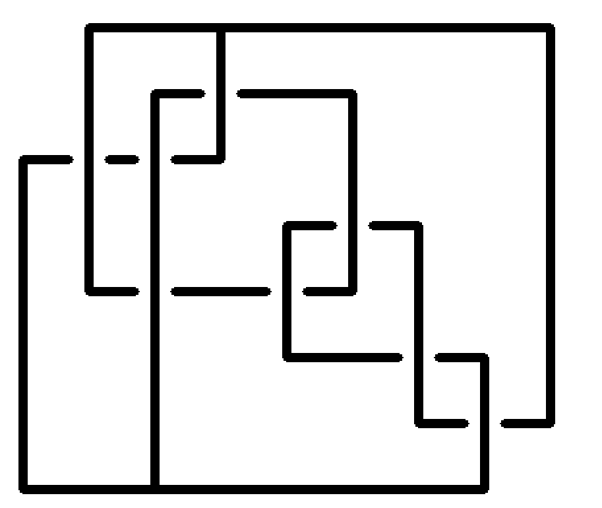
\includegraphics[width=\columnwidth]{C:/Users/io25j/Pictures/backup/documents/GitHub/R-E/Midterm_Poster/grid_diagram/theta_7_10.png}
    \caption{$7_{10}$} 
    \end{subfigure}
    \begin{subfigure}{0.075\textwidth}
    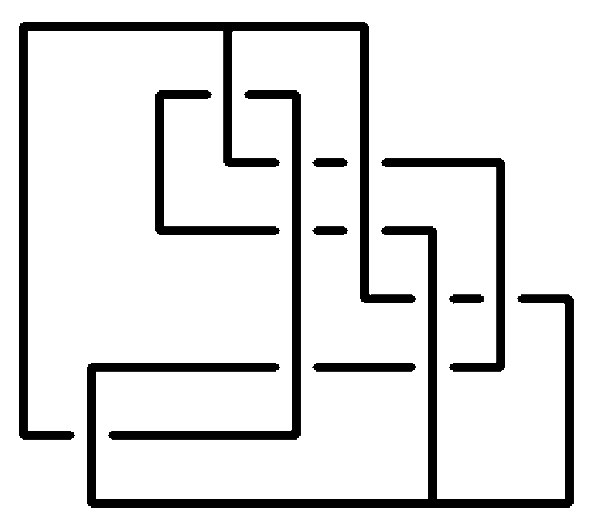
\includegraphics[width=\columnwidth]{C:/Users/io25j/Pictures/backup/documents/GitHub/R-E/Midterm_Poster/grid_diagram/theta_7_11.png}
    \caption{$7_{11}$} 
    \end{subfigure}
    \begin{subfigure}{0.075\textwidth}
    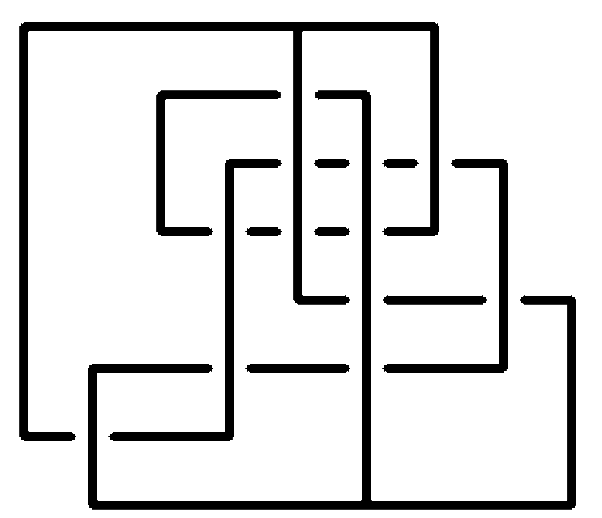
\includegraphics[width=\columnwidth]{C:/Users/io25j/Pictures/backup/documents/GitHub/R-E/Midterm_Poster/grid_diagram/theta_7_12.png}
    \caption{$7_{12}$} 
    \end{subfigure}
    \begin{subfigure}{0.075\textwidth}
    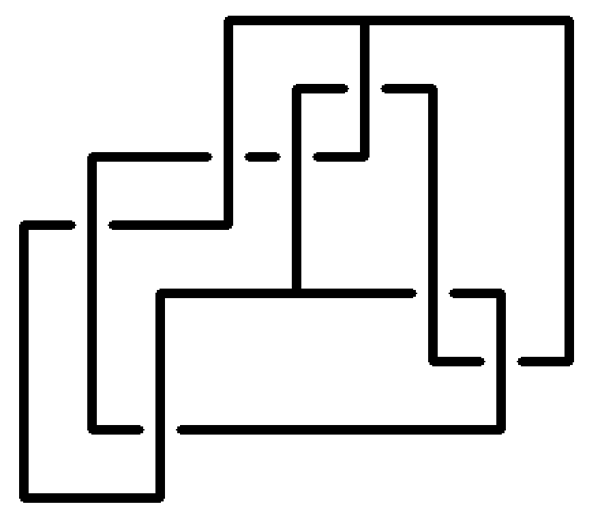
\includegraphics[width=\columnwidth]{C:/Users/io25j/Pictures/backup/documents/GitHub/R-E/Midterm_Poster/grid_diagram/theta_7_13.png}
    \caption{$7_{13}$} 
    \end{subfigure}
    \begin{subfigure}{0.075\textwidth}
    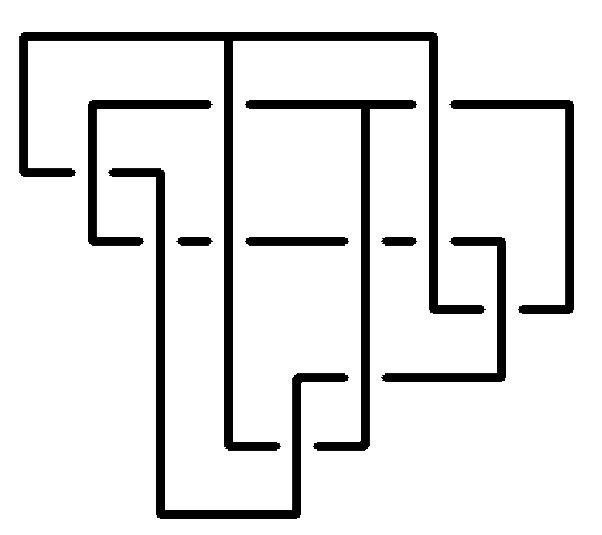
\includegraphics[width=\columnwidth]{C:/Users/io25j/Pictures/backup/documents/GitHub/R-E/Midterm_Poster/grid_diagram/theta_7_14.png}
    \caption{$7_{14}$} 
    \end{subfigure}
    \begin{subfigure}{0.075\textwidth}
    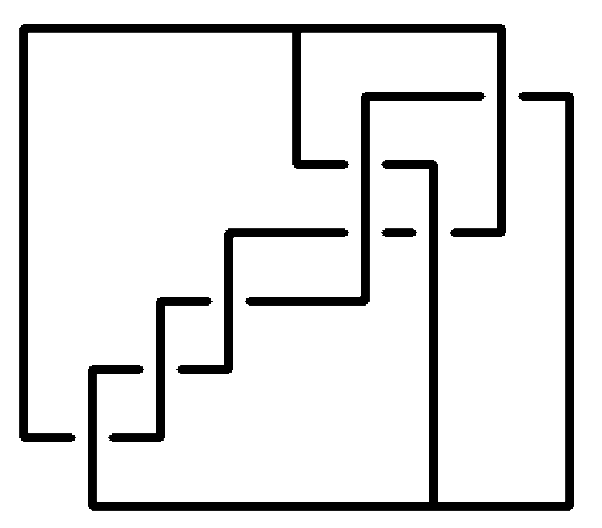
\includegraphics[width=\columnwidth]{C:/Users/io25j/Pictures/backup/documents/GitHub/R-E/Midterm_Poster/grid_diagram/theta_7_15.png}
    \caption{$7_{15}$} 
    \end{subfigure}
    \begin{subfigure}{0.075\textwidth}
    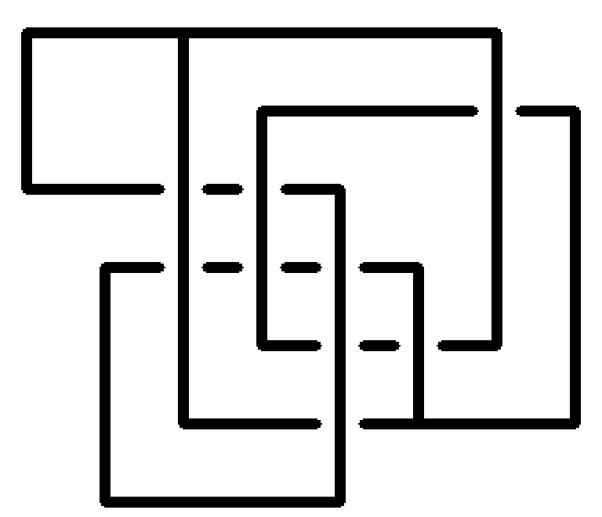
\includegraphics[width=\columnwidth]{C:/Users/io25j/Pictures/backup/documents/GitHub/R-E/Midterm_Poster/grid_diagram/theta_7_16.png}
    \caption{$7_{16}$} 
    \end{subfigure}
    \begin{subfigure}{0.075\textwidth}
    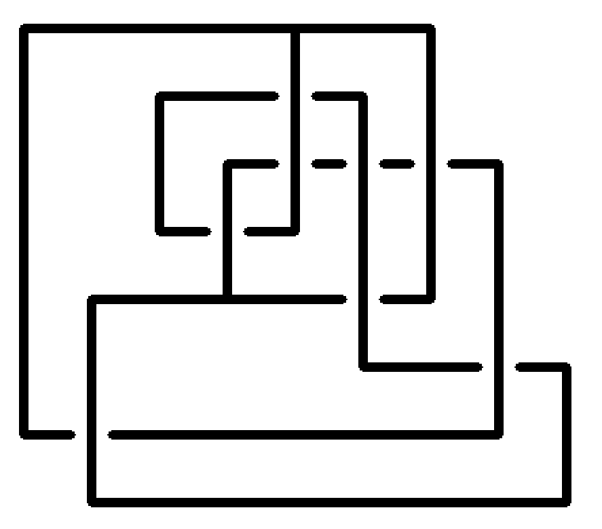
\includegraphics[width=\columnwidth]{C:/Users/io25j/Pictures/backup/documents/GitHub/R-E/Midterm_Poster/grid_diagram/theta_7_17.png}
    \caption{$7_{17}$} 
    \end{subfigure}
    \begin{subfigure}{0.075\textwidth}
    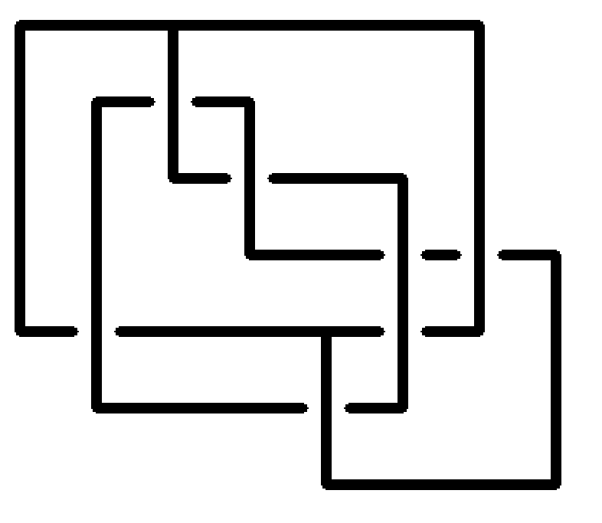
\includegraphics[width=\columnwidth]{C:/Users/io25j/Pictures/backup/documents/GitHub/R-E/Midterm_Poster/grid_diagram/theta_7_18.png}
    \caption{$7_{18}$} 
    \end{subfigure}
    \begin{subfigure}{0.075\textwidth}
    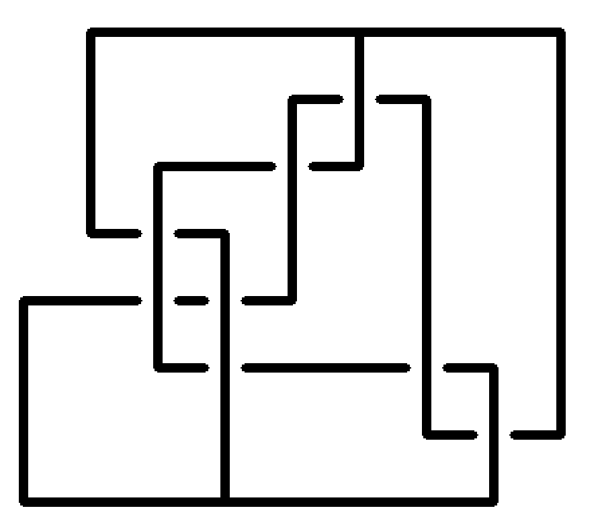
\includegraphics[width=\columnwidth]{C:/Users/io25j/Pictures/backup/documents/GitHub/R-E/Midterm_Poster/grid_diagram/theta_7_19.png}
    \caption{$7_{19}$} 
    \end{subfigure}
    \begin{subfigure}{0.075\textwidth}
    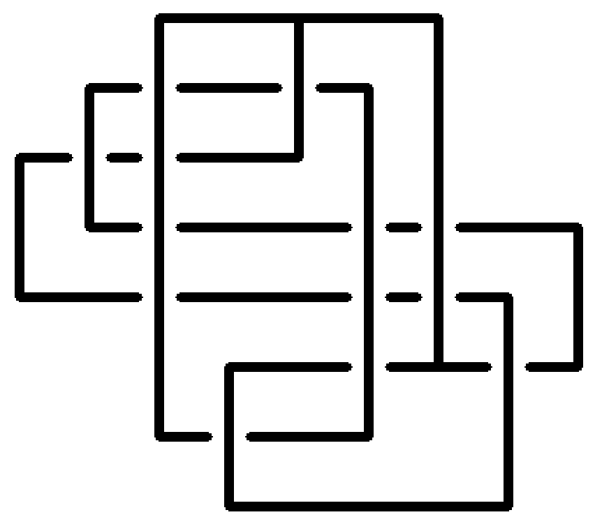
\includegraphics[width=\columnwidth]{C:/Users/io25j/Pictures/backup/documents/GitHub/R-E/Midterm_Poster/grid_diagram/theta_7_20.png}
    \caption{$7_{20}$} 
    \end{subfigure}
    \begin{subfigure}{0.075\textwidth}
    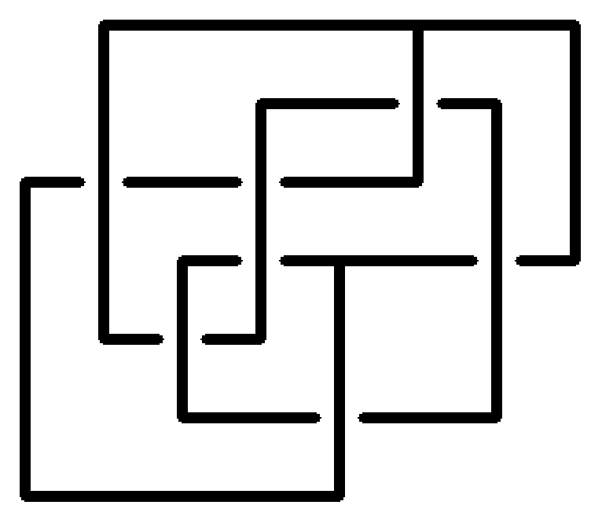
\includegraphics[width=\columnwidth]{C:/Users/io25j/Pictures/backup/documents/GitHub/R-E/Midterm_Poster/grid_diagram/theta_7_21.png}
    \caption{$7_{21}$} 
    \end{subfigure}
    \begin{subfigure}{0.075\textwidth}
    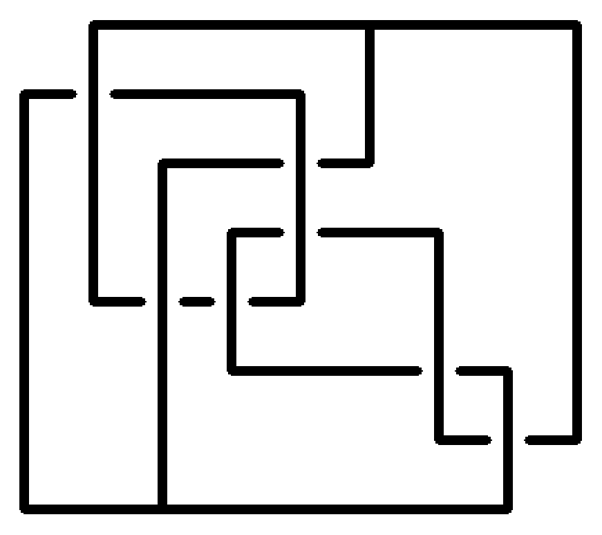
\includegraphics[width=\columnwidth]{C:/Users/io25j/Pictures/backup/documents/GitHub/R-E/Midterm_Poster/grid_diagram/theta_7_22.png}
    \caption{$7_{22}$} 
    \end{subfigure}
    \begin{subfigure}{0.075\textwidth}
    \includegraphics[width=\columnwidth]{C:/Users/io25j/Pictures/backup/documents/GitHub/R-E/Midterm_Poster/grid_diagram/theta_7_23.png}
    \caption{$7_{23}$} 
    \end{subfigure}
    \begin{subfigure}{0.075\textwidth}
    \includegraphics[width=\columnwidth]{C:/Users/io25j/Pictures/backup/documents/GitHub/R-E/Midterm_Poster/grid_diagram/theta_7_24.png}
    \caption{$7_{24}$} 
    \end{subfigure}
    \begin{subfigure}{0.075\textwidth}
    \includegraphics[width=\columnwidth]{C:/Users/io25j/Pictures/backup/documents/GitHub/R-E/Midterm_Poster/grid_diagram/theta_7_25.png}
    \caption{$7_{25}$} 
    \end{subfigure}
    \begin{subfigure}{0.075\textwidth}
    \includegraphics[width=\columnwidth]{C:/Users/io25j/Pictures/backup/documents/GitHub/R-E/Midterm_Poster/grid_diagram/theta_7_26.png}
    \caption{$7_{26}$} 
    \end{subfigure}
    \begin{subfigure}{0.075\textwidth}
    \includegraphics[width=\columnwidth]{C:/Users/io25j/Pictures/backup/documents/GitHub/R-E/Midterm_Poster/grid_diagram/theta_7_27.png}
    \caption{$7_{27}$} 
    \end{subfigure}
    \begin{subfigure}{0.075\textwidth}
    \includegraphics[width=\columnwidth]{C:/Users/io25j/Pictures/backup/documents/GitHub/R-E/Midterm_Poster/grid_diagram/theta_7_28.png}
    \caption{$7_{28}$} 
    \end{subfigure}
    \begin{subfigure}{0.075\textwidth}
    \includegraphics[width=\columnwidth]{C:/Users/io25j/Pictures/backup/documents/GitHub/R-E/Midterm_Poster/grid_diagram/theta_7_29.png}
    \caption{$7_{29}$} 
    \end{subfigure}





  \end{figure}


  \end{alertblock}
\end{column}
\begin{column}{0.5\textwidth}
  \begin{alertblock}{Handcuff Graphs}

  \end{alertblock}
  \end{column}
  \end{columns}

  \end{alertblock}

\begin{columns}[t]
  \column{0.33\textwidth}
  \begin{block}{Bounds of Arc Index}
    \begin{itemize}
      \item \textbf{Theta-curve} is a spatial knot on 3-sphere which has 2 vertices and 3 edges.
      In the projection of the theta-curve, the section where theta-curve meets itself is named \textbf{crossing}.
      If the one theta-curve and other theta-curve's continuous transform of the graph is same, these curves are \textbf{equivalent}.
      To transform a projection of theta-curve, the \textbf{generalized Reidemeister move} is used.
      \item \textbf{Handcuff graph} consists of two loops and an edge joining the loops.
      \item The \textbf{grid diagram} is made of horizontal lines and vertical lines, and vertical lines are always on top of horizontal lines.
      Except the vertices, two points that are bent vertically should be on each horizontal and vertical lines.
      The \textbf{Cromwell matrix} of theta-curve and handcuff graphs is the matrix made of 0 and 1.
      Except 2 rows, each row and columns has exactly two 1s, and for 2 rows, there are exactly three 1s.
      If the 1s are connected by horizontal and vertical lines, it leads to the grid diagram.
      The arc presentation can be expressed by grid diagram and vice versa.
      They are in one-to-one correspondence.
      Also, if the number of half planes are $\alpha$ on minimal arc presentation, the size of corresponding grid diagram is $(\alpha - 1) \times \alpha$.\\

    \end{itemize}
  \end{block}
  \column{0.33\textwidth}
  \begin{block}{새로운 거}
    새로운 거
  \end{block}
  \column{0.33\textwidth}
  \begin{block}{새로운 거}

    This block catches your eye, so \textbf{important stuff} should probably go
    here.

    Curabitur eu libero vehicula, cursus est fringilla, luctus est. Morbi
    consectetur mauris quam, at finibus elit auctor ac. Aliquam erat volutpat.
    Aenean at nisl ut ex ullamcorper eleifend et eu augue. Aenean quis velit
    tristique odio convallis ultrices a ac odio.

    \begin{itemize}
      \item \textbf{Fusce dapibus tellus} vel tellus semper finibus. In
        consequat, nibh sed mattis luctus, augue diam fermentum lectus.
      \item \textbf{In euismod erat metus} non ex. Vestibulum luctus augue in
        mi condimentum, at sollicitudin lorem viverra.
      \item \textbf{Suspendisse vulputate} mauris vel placerat consectetur.
        Mauris semper, purus ac hendrerit molestie, elit mi dignissim odio, in
        suscipit felis sapien vel ex.
    \end{itemize}

    Aenean tincidunt risus eros, at gravida lorem sagittis vel. Vestibulum ante
    ipsum primis in faucibus orci luctus et ultrices posuere cubilia Curae.

  \end{block}
\end{columns}



% \end{columns}
\end{frame}

\end{document}
